\chapter{Evaluation}
\label{ch:evaluation}

\begin{draft}
GLMTK by me was used for evaluation.
Commit before bachelor-thesis release.

Experiment to showcase (dis-)advantages of GLM to MKN.

Maybe Speedup-factor over time.

Experiments that combine metrices.

Experiments over time and space complexity.
\end{draft}

% ------------------------------------------------------------------------------
\section{Normalized Keystroke Savings}

\begin{draft}
How are they defined?
How do we calculate them?

From \textcite{Trnka2011}:
\begin{equation}
  \frac{\text{keystrokes}_\text{normal} - \text{keystrokes}_\text{with prediction}}
       {\text{keystrokes}_\text{normal}}
\end{equation}
We differ on how we count spaces, newlines, etc...
No keystroke for accepting completion.

\end{draft}

% ------------------------------------------------------------------------------
\section{Experimental setup}

\begin{draft}
Computer.

Corpora.
\textcite{OANC}
How to tokenize corpus?
Hard to without semantic knowledge.
Currently: all special characters are surrounded by spaces.
But \texttt{you're} becomes \texttt{you ' re}.
No stemming to normalize word forms.
Case-sensitive training and test data.
Kept names.

How to scale completion trie depth for word prediction experiments?
Remove sentences from corpus?
Remove entries of from completion trie?

Avoid unknown words / unknown ngrams in testing?

Because of JVM experiments need to be run multiple times.
Graphs then show average + variance (or rather standard deviation)?

How to calculate standard derivation?
Use \emph{sample standard deviation}?
Why divide by $N-1$ there?
\end{draft}

% ------------------------------------------------------------------------------
\section{Probability calculation}

\begin{draft}
Experiment: Calculate one probability $\Prob{w_n}{w_1^{n-1}}$ with MKN and GLM
for recursive and weighted sum implementations for increasing $n$ and track
execution time.

Experiment: Calculate one probability $\Prob{w_n}{w_1^{n-1}}$ with weighted sum
MKN and GLM for increasing $n$ and track execution times of $\SumWeight^h_i$
calculation and remaining calculations.

For different percentages of seen sequences?

To showcase usefulness of weighted sum approach.

WSA as maximal optimization / baseline.
What is WSA again?

Number of weights per model.
\end{draft}

\begin{figure}
  \hspace{-5em}
  \centering
  \begin{subfigure}{.45\textwidth}
    \documentclass{standalone}
\usepackage[dvipsnames,svgnames,x11names]{xcolor}
\usepackage{tikz}
\usepackage{pgfplots}
\pgfplotsset{compat = 1.12}
\usepackage{../thesismath}
\begin{document}
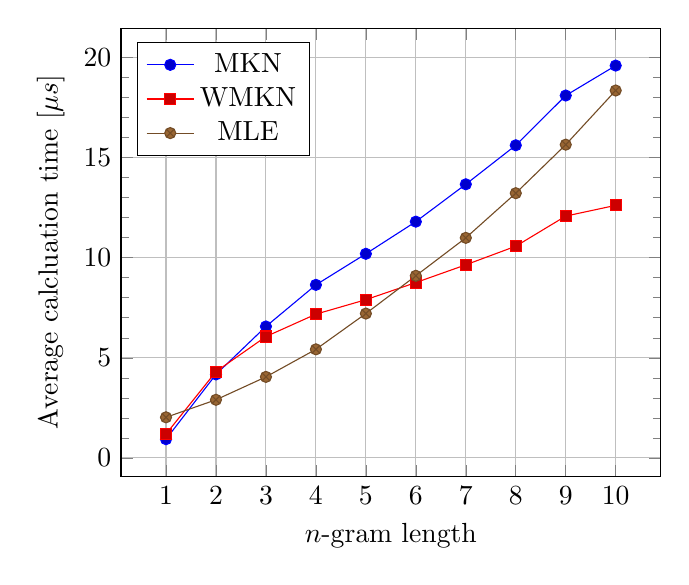
\begin{tikzpicture}[baseline]

\begin{axis}[
  xlabel = {$n$-gram length},
  xtick = {1, ..., 10},
  ylabel = {Average calcluation time [${\mu}s$]},
  minor y tick num = 4,
  grid = major,
  legend entries = {{MKN}, {WMKN}, {MLE}},
  legend pos = north west,
]

% MKN
\addplot table {
  n   us
  % sampled at N = 1000
  1    0.936
  2    4.171
  3    6.565
  4    8.643
  5   10.194
  6   11.800
  7   13.666
  8   15.614
  9   18.099
  10  19.594
};

% WMKN
\addplot table {
  n   us
  % sampled at N = 1000
  1    1.192
  2    4.311
  3    6.060
  4    7.180
  5    7.902
  6    8.758
  7    9.644
  8   10.573
  9   12.078
  10  12.614
};

% MKN
\addplot table {
  n   us
  % sampled at N = 1000
  1    2.028
  2    2.903
  3    4.047
  4    5.423
  5    7.210
  6    9.096
  7   10.991
  8   13.221
  9   15.645
  10  18.350
};

\end{axis}

\end{tikzpicture}
\end{document}

  \end{subfigure}
  \hspace{4em}
  \begin{subfigure}{.45\textwidth}
    \documentclass{standalone}
\usepackage[dvipsnames,svgnames,x11names]{xcolor}
\usepackage{tikz}
\usepackage{pgfplots}
\pgfplotsset{compat = 1.12}
\usepackage{../thesismath}
\begin{document}
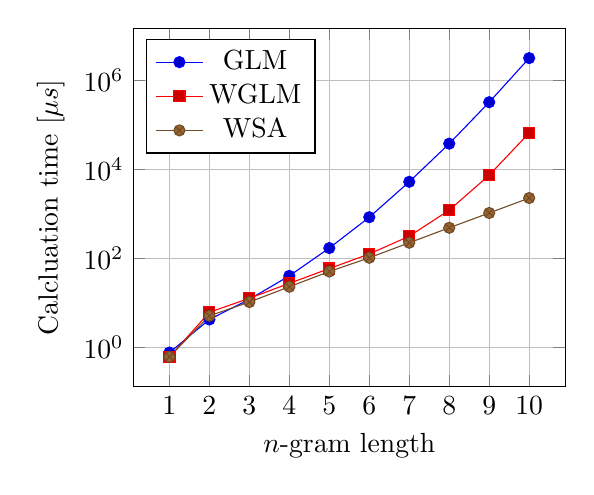
\begin{tikzpicture}[baseline]

\begin{axis}[
  xlabel = {$n$-gram length},
  xtick = {1, ..., 10},
  ylabel = {Calcluation time [${\mu}s$]},
  ymode = log,
  %yticklabel pos = right,
  minor y tick num = 4,
  grid = major,
  legend entries = {{GLM}, {WGLM}, {WSA}},
  legend pos = north west,
  scale = 0.8,
]

% GLM
\addplot table {
  n   us
  % sampled at N = 1000
  1   0.776
  2   4.296
  3   12.188
  4   40.981
  5   172.271
  % sampled at N = 100
  6   848.550
  7   5297.308
  % sampled at N = 10
  8   38045.228
  9   323947.490
  % sampled at N = 1
  10  3168612.887
};

% WGLM
\addplot table {
  n   us
  % sampled at N = 1000
  1   0.618
  2   6.223
  3   12.855
  4   27.786
  5   59.746
  % sampled at N = 100
  6   126.934
  7   317.936
  8   1223.680
  9   7463.531
  10  66226.605
};

% WSA
\addplot table {
  n   us
  % sampled at N = 1000
  1   0.624
  2   5.200
  3   10.572
  4   23.295
  5   51.307
  % sampled at N = 100
  6   104.217
  7   226.905
  8   491.327
  9   1056.845
  10  2287.351
};

\end{axis}

\end{tikzpicture}
\end{document}

  \end{subfigure}
  \caption{TimeMKN+TimeGLM-Caption}
\end{figure}

% ------------------------------------------------------------------------------
\section{Word prediction calculation}

\begin{draft}
Experiment: top-$1$ word prediction with na\"{\i}ve method, TA and NRA scale
trie depth track execution time and space requirements.

Experiment: top-$k$ word prediction with na\"{\i}ve method, TA and NRA scale
$k$ track execution time and space requirements.

Experiment: NKSS calculation with na\"{\i}ve method, TA and NRA for some fixed
$k$ scale completion trie depth.

Experiment with prefix?

How many words in vocab does each algorithm compute probability of?

All experiments for MKN and GLM?
Probably yes, to see if difference matters.

Completion Trie memory consumption relevant?

Random access from completion trie or from hash map?

Mention decreasingness (?) of data sets.
\end{draft}

% ------------------------------------------------------------------------------
\section{Word prediction quality}

\begin{draft}
Is this section relevant for this thesis?

Experiment: NKSS quality of MKN vs GLM prediction for different $n$ and corpus
sizes.
\end{draft}
